
\begin{frame}{Kết quả thực nghiệm}
    \small
    \begin{table}[]
        \centering
        \caption{So sánh hiệu năng trên tập kiểm tra}
        \resizebox{0.5\textwidth}{!}{%
        \begin{tabular}{lccccc}
        \hline
        \textbf{Mô hình} & \textbf{PSNR (dB) $\uparrow$} & \textbf{NMSE $\downarrow$} & \textbf{SSIM $\uparrow$} & \textbf{Tham số} & \textbf{FPS} \\ \hline
        GAN & 28.74 & 0.006 & 0.842 & 14.59M & 188 \\ 
        Flow-based & 27.09 & 0.008 & 0.831 & 25.87M & 35 \\ 
        AE2 & 27.79 & 0.007 & 0.840 & 0.375M & 411 \\ 
        AE3 & 26.16 & 0.011 & 0.802 & 2.77M & 289 \\ 
        AE4 & 29.40 & 0.005 & 0.864 & 14.59M & 189 \\ 
        AE5 & 27.24 & 0.008 & 0.793 & 48.43M & 119 \\ \hline
        VRAE2 & 30.32 & 0.004 & 0.884 & 0.376M & 399 \\ 
        \textbf{VRAE3} & \textbf{31.05} & \textbf{0.003} & \textbf{0.898} & \textbf{2.78M} & \textbf{194} \\ 
        VRAE4 & 30.25 & 0.004 & 0.880 & 14.61M & 90 \\ 
        VRAE5 & 30.03 & 0.003 & 0.860 & 48.48M & 45 \\ \hline
        \end{tabular}%
        }
    \end{table}
    \textbf{Nhận xét:}
    \begin{itemize}
        \item \textbf{VRAE3} đạt kết quả tốt nhất: PSNR 31.05 dB, SSIM 0.898
        \item So với AE cùng độ sâu: Cải thiện PSNR ~20\%, giảm NMSE ~50\%, tăng SSIM ~1\%
        \item Chỉ tăng tham số không đáng kể (~1\%) nhưng cải thiện đáng kể chất lượng
    \end{itemize}
\end{frame}

% \begin{frame}{So sánh với các phương pháp cơ sở}
%     \small
%     \begin{itemize}
%         \item \textbf{Độ chính xác tái tạo:} VRAE3 vượt trội ở cả PSNR, SSIM và NMSE
%         \begin{itemize}
%             \item PSNR: +2.31 dB so với GAN, +4.89 dB so với FB, +4.89 dB so với AE3
%             \item SSIM: +0.056 so với GAN, cao hơn hầu hết các phương pháp
%         \end{itemize}
%         \item \textbf{Hiệu năng tính toán:}
%         \begin{itemize}
%             \item VRAE2: 399 FPS (rất phù hợp thời gian thực)
%             \item VRAE3: 194 FPS với chất lượng tốt nhất
%             \item Cân bằng tốt giữa chất lượng và tốc độ
%         \end{itemize}
%         \item \textbf{Hiệu quả tham số:} VRAE đạt chất lượng cao với số tham số tương đương AE
%     \end{itemize}
% \end{frame}

\begin{frame}{Phân tích Entropy}
    \begin{columns}
        \begin{column}{0.5\textwidth}
            \begin{figure}
                \centering
                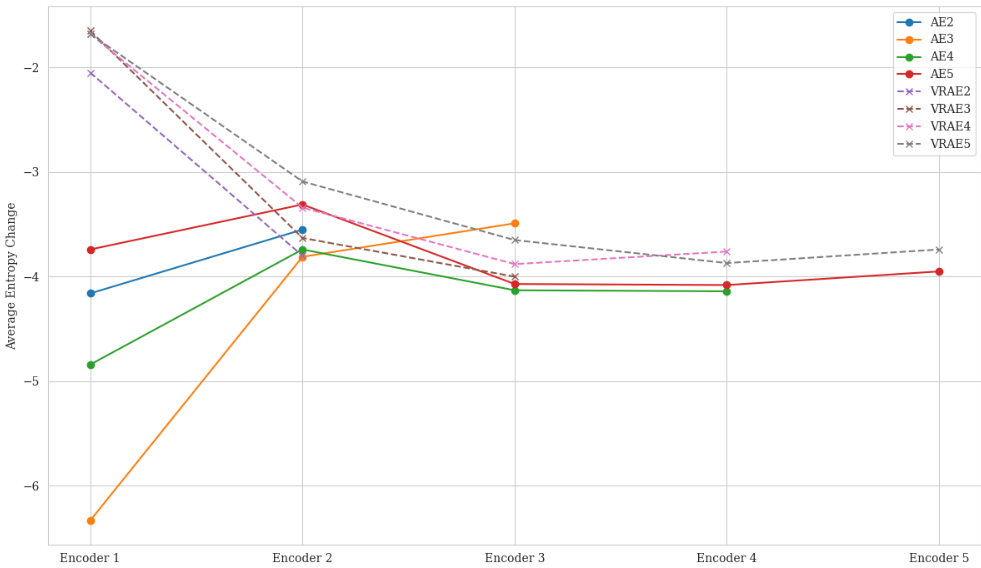
\includegraphics[width=\linewidth]{images/entropy_change.png}
                \caption{Thay đổi Entropy qua các lớp mã hóa}
            \end{figure}
        \end{column}
        \begin{column}{0.5\textwidth}
            \textbf{Quan sát:}
            \begin{itemize}
                \item \textbf{Giai đoạn đầu:} VRAE bắt đầu với mức entropy cao hơn AE
                \item Bảo toàn được nhiều đặc trưng thô và chi tiết vi mô ngay từ đầu
                \item \textbf{Sự ổn định:} Giảm entropy mượt mà, nhất quán
                \item Tránh "sụp đổ thông tin" (information collapse) quá sớm
            \end{itemize}
            
            \textbf{Ví dụ VRAE3:}
            \begin{itemize}
                \item Giảm dần: -1.5 $\rightarrow$ -3.7
                \item Trái ngược AE3: -6.3 $\rightarrow$ -3.5 (giảm đột ngột)
            \end{itemize}
        \end{column}
    \end{columns}
\end{frame}

% \begin{frame}{Phân tích Trade-off (Pareto Front)}
%     \begin{columns}
%         \begin{column}{0.5\textwidth}
%             \begin{figure}
%                 \centering
%                 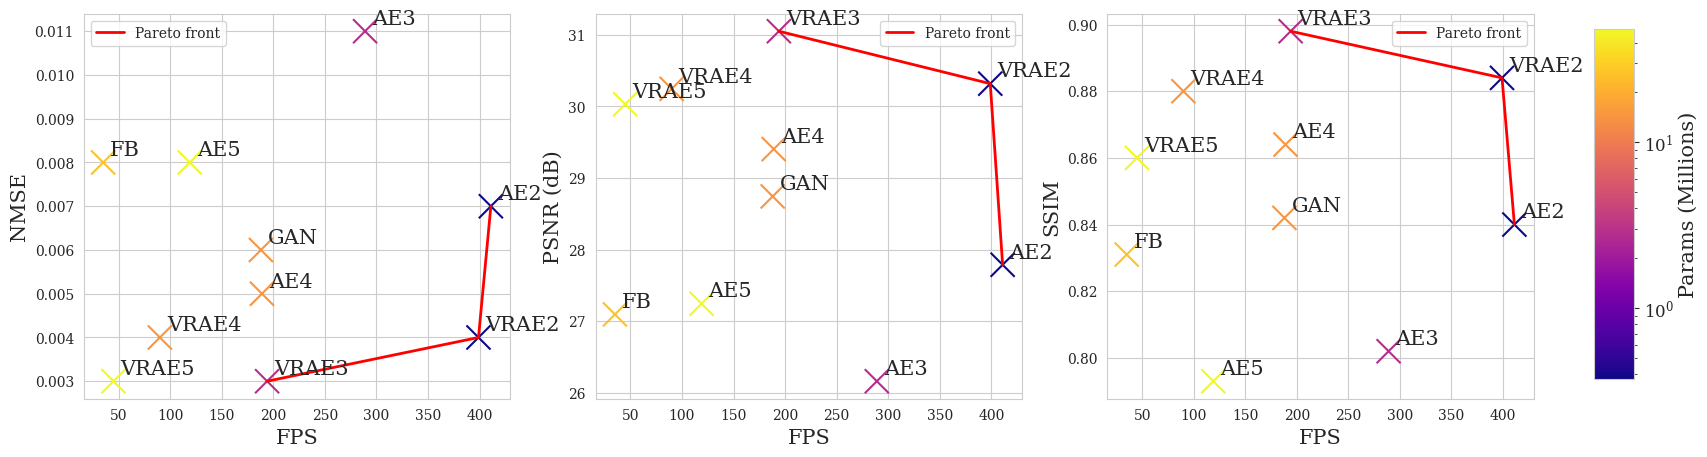
\includegraphics[width=\linewidth]{images/pareto.png}
%                 \caption{Pareto Front: Chất lượng vs Tốc độ}
%             \end{figure}
%         \end{column}
%         \begin{column}{0.5\textwidth}
%             \textbf{Đánh đổi giữa:}
%             \begin{itemize}
%                 \item Hiệu suất tái tạo (PSNR/SSIM)
%                 \item Tốc độ suy luận (FPS)
%             \end{itemize}
            
%             \vspace{0.3cm}
%             \textbf{Kết quả:}
%             \begin{itemize}
%                 \item VRAE2 và VRAE3 nằm trên \textbf{đường biên tối ưu}
%                 \item Kết hợp tốt nhất giữa độ chính xác và hiệu năng
%                 \item GAN và FB: Tham số lớn nhưng hiệu quả thấp hơn
%             \end{itemize}
%         \end{column}
%     \end{columns}
% \end{frame}

